\chapter*{Prefazione}
\addcontentsline{toc}{chapter}{Prefazione}

\section*{L'arte degli algoritmi}

L'informatica moderna è fondata su due pilastri fondamentali: gli \textbf{algoritmi} e le \textbf{strutture dati}. Un algoritmo è una sequenza finita di istruzioni ben definite che, dato un input, produce un output risolvendo un problema computazionale. Le strutture dati, d'altra parte, sono modi organizzati di memorizzare e gestire i dati in modo che possano essere utilizzati efficacemente.

La relazione tra questi due concetti è profonda e inscindibile: un algoritmo efficiente richiede strutture dati appropriate, e viceversa, strutture dati sofisticate hanno senso solo nel contesto di algoritmi che le sfruttano adeguatamente.

\section*{Scopo di questo testo}

Questo libro nasce con l'obiettivo di fornire una trattazione rigorosa ma accessibile dei fondamenti teorici e pratici degli algoritmi e delle strutture dati. Il testo è strutturato per essere utilizzato sia come manuale di studio per corsi universitari, sia come riferimento per professionisti che desiderano approfondire le proprie conoscenze.

Gli obiettivi principali sono:

\begin{enumerate}
    \item \textbf{Rigore matematico}: Ogni concetto è introdotto con definizioni formali e, quando appropriato, corredato da teoremi e dimostrazioni. La matematica non è un ornamento, ma lo strumento essenziale per comprendere le proprietà degli algoritmi.

    \item \textbf{Analisi di complessità}: Un algoritmo non è "buono" o "cattivo" in astratto, ma in relazione al suo costo computazionale. Dedicheremo ampio spazio all'analisi asintotica e ai diversi scenari (caso migliore, medio, peggiore).

    \item \textbf{Implementabilità}: Ogni struttura dati e algoritmo è presentato con pseudocodice dettagliato, facilmente traducibile in linguaggi di programmazione reali.

    \item \textbf{Visualizzazione}: Diagrammi, alberi e grafi sono rappresentati graficamente usando TikZ per facilitare la comprensione intuitiva dei concetti.

    \item \textbf{Applicazioni pratiche}: Oltre alla teoria, vengono discusse le applicazioni reali e i casi d'uso di ogni struttura dati e algoritmo presentato.
\end{enumerate}

\section*{Prerequisiti}

Per trarre il massimo beneficio da questo testo, il lettore dovrebbe possedere:

\begin{itemize}
    \item \textbf{Matematica di base}: Familiarità con algebra elementare, logaritmi, esponenziali, e nozioni di base di teoria degli insiemi.

    \item \textbf{Matematica discreta}: Conoscenza di elementi di logica matematica, tecniche di dimostrazione (induzione, dimostrazione per assurdo), combinatoria elementare.

    \item \textbf{Programmazione}: Esperienza con almeno un linguaggio di programmazione imperativo o orientato agli oggetti. La conoscenza di concetti come variabili, cicli, condizionali, funzioni e ricorsione è essenziale.

    \item \textbf{Curiosità intellettuale}: Forse il prerequisito più importante. Gli algoritmi sono oggetti di grande bellezza matematica, e lo studio di questo campo richiede pazienza e desiderio di comprendere in profondità.
\end{itemize}

\section*{Notazione matematica}

In questo testo utilizzeremo una notazione matematica standard. Ecco alcune convenzioni importanti:

\begin{itemize}
    \item $\mathbb{N}$ denota l'insieme dei numeri naturali $\{0, 1, 2, 3, \ldots\}$
    \item $\mathbb{Z}$ denota l'insieme dei numeri interi $\{\ldots, -2, -1, 0, 1, 2, \ldots\}$
    \item $\mathbb{R}$ denota l'insieme dei numeri reali
    \item $\mathbb{R}^+$ denota l'insieme dei numeri reali positivi
    \item $\lg n$ denota il logaritmo in base 2 di $n$ (logaritmo binario)
    \item $\ln n$ denota il logaritmo naturale di $n$ (base $e$)
    \item $\log n$ denota generalmente $\lg n$ in contesti algoritmici
    \item $\lfloor x \rfloor$ denota la parte intera inferiore di $x$ (floor)
    \item $\lceil x \rceil$ denota la parte intera superiore di $x$ (ceiling)
    \item $n!$ denota il fattoriale di $n$: $n! = n \cdot (n-1) \cdot (n-2) \cdots 2 \cdot 1$
    \item $\binom{n}{k}$ denota il coefficiente binomiale: $\frac{n!}{k!(n-k)!}$
\end{itemize}

Per le sommatorie e i prodotti utilizzeremo:

\[
\sum_{i=1}^{n} f(i) = f(1) + f(2) + \cdots + f(n)
\]

\[
\prod_{i=1}^{n} f(i) = f(1) \cdot f(2) \cdots f(n)
\]

Alcune sommatorie importanti che ricorreranno frequentemente:

\begin{align*}
\sum_{i=1}^{n} i &= \frac{n(n+1)}{2} = \Theta(n^2) \\
\sum_{i=1}^{n} i^2 &= \frac{n(n+1)(2n+1)}{6} = \Theta(n^3) \\
\sum_{i=0}^{n} 2^i &= 2^{n+1} - 1 = \Theta(2^n) \\
\sum_{i=0}^{n} r^i &= \frac{r^{n+1}-1}{r-1} \quad \text{per } r \neq 1 \\
\sum_{i=1}^{n} \frac{1}{i} &= \ln n + O(1) \quad \text{(serie armonica)}
\end{align*}

\section*{Pseudocodice}

Gli algoritmi in questo testo sono presentati usando uno pseudocodice che mescola elementi di notazione matematica e costrutti di programmazione imperativi. Lo pseudocodice è progettato per essere:

\begin{itemize}
    \item \textbf{Leggibile}: Deve essere comprensibile anche a chi non conosce un linguaggio di programmazione specifico.
    \item \textbf{Preciso}: Deve specificare esattamente cosa fa l'algoritmo, senza ambiguità.
    \item \textbf{Traducibile}: Deve poter essere facilmente convertito in codice eseguibile.
\end{itemize}

Convenzioni dello pseudocodice:

\begin{itemize}
    \item L'\textbf{indentazione} indica la struttura dei blocchi
    \item \texttt{if-then-else}, \texttt{while}, \texttt{for} hanno il significato usuale
    \item \texttt{return} termina l'esecuzione e restituisce un valore
    \item Gli \textbf{array} sono indicizzati da 1 (salvo diversa indicazione)
    \item L'accesso a un elemento dell'array $A$ di indice $i$ è scritto come $A[i]$
    \item L'assegnamento è indicato con $\leftarrow$
    \item Il confronto di uguaglianza è indicato con $=$
    \item I commenti sono preceduti da \texttt{//}
\end{itemize}

Esempio di pseudocodice:

\begin{lstlisting}[style=pseudocode]
def SommaArray(A, n):
    """
    Calcola la somma degli elementi di un array
    Input: array A di n elementi
    Output: somma degli elementi
    """
    somma = 0
    for i = 1 to n:
        somma = somma + A[i]
    return somma
\end{lstlisting}

\section*{Struttura del libro}

Il testo è organizzato in capitoli progressivi, ciascuno dei quali si basa sui concetti introdotti nei precedenti:

\begin{description}
    \item[Capitolo 1: Introduzione e Complessità] Introduciamo le notazioni asintotiche (Big-O, Omega, Theta) e i metodi per analizzare la complessità temporale e spaziale degli algoritmi. Discutiamo i casi migliore, medio e peggiore.

    \item[Capitolo 2: Array e Liste] Esaminiamo le strutture dati fondamentali: array (statici e dinamici) e liste concatenate (semplici, doppie, circolari). Analizziamo le operazioni di base e le loro complessità.

    \item[Capitolo 3: Stack e Code] Studiamo due strutture dati lineari fondamentali: stack (LIFO) e queue (FIFO), con le loro varianti e applicazioni pratiche come valutazione di espressioni e gestione di processi.

    \item[Capitolo 4: Alberi] Approfondiamo gli alberi binari, alberi binari di ricerca (BST), alberi AVL (auto-bilancianti) e heap. Analizziamo le operazioni di inserimento, cancellazione e ricerca.

    \item[Capitolo 5: Grafi] Introduciamo i grafi, le loro rappresentazioni (matrice di adiacenza, lista di adiacenza), e algoritmi fondamentali come BFS, DFS, e algoritmi per cammini minimi (Dijkstra, Bellman-Ford).

    \item[Capitolo 6: Tabelle Hash] Studiamo le funzioni hash, la gestione delle collisioni tramite concatenamento (chaining) e indirizzamento aperto (open addressing), e l'analisi delle prestazioni.

    \item[Capitolo 7: Algoritmi di Ordinamento] Analizziamo algoritmi di ordinamento classici: Bubble Sort, Insertion Sort, Merge Sort, Quick Sort, Heap Sort, con confronto delle complessità.

    \item[Capitolo 8: Algoritmi di Ricerca] Studiamo la ricerca lineare e binaria, alberi di ricerca ottimali, e strutture dati avanzate per la ricerca.

    \item[Capitolo 9: Ricorsione] Approfondiamo la ricorsione, le relazioni di ricorrenza, il Master Theorem, e tecniche per risolvere equazioni di ricorrenza.

    \item[Capitolo 10: Programmazione Dinamica] Introduciamo il paradigma della programmazione dinamica, con esempi classici come il problema dello zaino, il calcolo di Fibonacci, e la longest common subsequence.

    \item[Capitolo 11: Algoritmi Greedy] Studiamo gli algoritmi greedy (golosi) e le loro proprietà: scelta greedy, sottostruttura ottima. Esempi: problema dello zaino frazionario, algoritmo di Huffman.

    \item[Capitolo 12: Backtracking] Esploriamo la tecnica del backtracking per problemi di ricerca esaustiva: N-regine, Sudoku, percorsi in grafi.
\end{description}

\section*{Come usare questo libro}

Questo testo può essere utilizzato in diversi modi:

\begin{itemize}
    \item \textbf{Corso universitario}: I capitoli sono pensati per coprire un semestre di un corso di Algoritmi e Strutture Dati. Ogni capitolo può corrispondere a 1-2 settimane di lezioni.

    \item \textbf{Studio individuale}: I capitoli sono auto-contenuti e possono essere studiati indipendentemente, anche se è consigliabile seguire l'ordine proposto. Ogni concetto è spiegato da zero.

    \item \textbf{Riferimento rapido}: Le definizioni formali, i teoremi e gli pseudocodici possono servire come riferimento rapido per chi ha già familiarità con gli argomenti.

    \item \textbf{Preparazione a colloqui tecnici}: Le sezioni sulle applicazioni pratiche e gli esercizi possono essere utili per prepararsi a colloqui di lavoro nel settore informatico.
\end{itemize}

\section*{Consigli per lo studio}

Studiare algoritmi e strutture dati richiede un approccio attivo. Ecco alcuni consigli:

\begin{enumerate}
    \item \textbf{Non limitarsi a leggere}: Cerca di implementare gli algoritmi in un linguaggio di programmazione. Solo scrivendo codice si comprende davvero il funzionamento degli algoritmi.

    \item \textbf{Seguire le dimostrazioni}: Le dimostrazioni dei teoremi non sono opzionali. Contengono l'essenza della comprensione. Se una dimostrazione non è chiara, rileggila, scrivila su carta, discutila con altri.

    \item \textbf{Visualizzare}: Disegna alberi, grafi, traccia l'esecuzione degli algoritmi passo passo. La visualizzazione aiuta enormemente la comprensione.

    \item \textbf{Fare esercizi}: La comprensione teorica deve essere consolidata con esercizi pratici. Implementa le varianti, risolvi problemi, analizza nuovi algoritmi.

    \item \textbf{Confrontare alternative}: Per ogni problema, considera diverse soluzioni e confrontale in termini di complessità temporale, spaziale, semplicità di implementazione.

    \item \textbf{Approfondire}: Questo libro è un'introduzione. Per ogni argomento esistono trattazioni più avanzate. Usa la bibliografia per esplorare ulteriormente.
\end{enumerate}

\section*{Bibliografia essenziale}

Questo testo si basa su decenni di ricerca e didattica nel campo degli algoritmi. Alcune opere di riferimento fondamentali:

\begin{itemize}
    \item \textbf{Cormen, Leiserson, Rivest, Stein}: \textit{Introduction to Algorithms} (4a ed.). Il testo di riferimento per eccellenza, completo e rigoroso.

    \item \textbf{Knuth, Donald}: \textit{The Art of Computer Programming} (volumi 1-4A). L'opera monumentale che ha definito il campo.

    \item \textbf{Sedgewick, Wayne}: \textit{Algorithms} (4a ed.). Eccellente per le implementazioni pratiche e la visualizzazione.

    \item \textbf{Kleinberg, Tardos}: \textit{Algorithm Design}. Ottimo per le tecniche di progettazione di algoritmi.

    \item \textbf{Skiena, Steven}: \textit{The Algorithm Design Manual} (3a ed.). Ricco di esempi pratici e war stories.

    \item \textbf{Aho, Hopcroft, Ullman}: \textit{Data Structures and Algorithms}. Un classico intramontabile.
\end{itemize}

\section*{Ringraziamenti}

Lo studio degli algoritmi è un viaggio intellettuale che non si compie mai in solitudine. Questo testo è il frutto di innumerevoli discussioni, lezioni, letture e riflessioni.

Ringrazio i pionieri del campo---Dijkstra, Knuth, Hoare, Tarjan, Floyd, e tanti altri---le cui idee brillanti sono diventate patrimonio comune dell'informatica. Ringrazio i docenti che hanno reso accessibile questa materia complessa, e gli studenti le cui domande hanno stimolato chiarimenti e approfondimenti.

Questo libro è dedicato a chiunque sia affascinato dalla bellezza matematica degli algoritmi e voglia comprendere come piccole sequenze di istruzioni possano risolvere problemi di enorme complessità.

\section*{Nota finale}

Gli algoritmi non sono solo oggetti di studio accademico. Ogni volta che usiamo un motore di ricerca, un navigatore GPS, un social network, un sistema di raccomandazione, stiamo beneficiando di algoritmi sofisticati che operano dietro le quinte.

Comprendere gli algoritmi significa comprendere i fondamenti del mondo digitale in cui viviamo. È un potere intellettuale che apre porte, sia professionali che culturali.

Buono studio, e benvenuti nel meraviglioso mondo degli algoritmi e delle strutture dati.

\vspace{1cm}

\hfill \textit{L'Autore}

\vspace{2cm}

\begin{center}
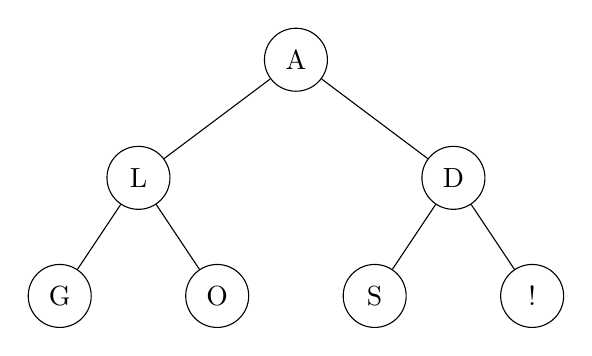
\begin{tikzpicture}[
    level distance=1.5cm,
    level 1/.style={sibling distance=4cm},
    level 2/.style={sibling distance=2cm},
    every node/.style={circle, draw, minimum size=0.8cm}
]
\node {A}
    child {node {L}
        child {node {G}}
        child {node {O}}
    }
    child {node {D}
        child {node {S}}
        child {node {!}}
    };
\end{tikzpicture}

\small \textit{Un albero per iniziare il viaggio...}
\end{center}

